%%%%%%%%%%%%%%%%%%%%%%%%%%%%%%%%%%%%%%%%%%%%%%%%%%%%%%%%%%%%%%%%%%%%%%%%
\chapter{Financiële haalbaarheid}
%%%%%%%%%%%%%%%%%%%%%%%%%%%%%%%%%%%%%%%%%%%%%%%%%%%%%%%%%%%%%%%%%%%%%%%%

\begin{center}
  \begin{minipage}{0.5\textwidth}
    \begin{small}
    \end{small}
  \end{minipage}
  \vspace{0.5cm}
\end{center}

%%%%%%%%%%%%%%%%%%%%%%%%%%%%%%%%%%%%%%%%%%%%%%%%%%%%%%%%%%%%%%%%%%%%%%%%
\section{Inleiding}
%%%%%%%%%%%%%%%%%%%%%%%%%%%%%%%%%%%%%%%%%%%%%%%%%%%%%%%%%%%%%%%%%%%%%%%%

Het uitschrijven van één uur geluid kost ongeveer 8 á 10 uur werk en is dus erg arbeidsintensief en dus erg duur. Automatische spraakherkenning (ASR = Automatic Speech Recognition) is snel en erg goedkoop, maar helaas maken de spraakherkenningsprogramma’s nog wel veel fouten. In de toekomst zal dit zeker beter gaan, maar op dit moment worden ongeveer 20% van de woorden nog niet goed herkend.%%%%%%%%%%%%%%%%%%%%%%%%%%%%%%%%%%%%%%%%%%%%%%%%%%%%%%%%%%%%%%%%%%%%%%%%

%%%%%%%%%%%%%%%%%%%%%%%%%%%%%%%%%%%%%%%%%%%%%%%%%%%%%%%%%%%%%%%%%%%%%%%%
\section{Financiële parameters}
%%%%%%%%%%%%%%%%%%%%%%%%%%%%%%%%%%%%%%%%%%%%%%%%%%%%%%%%%%%%%%%%%%%%%%%%
De prijzen die zijn uitgelijnd in deze paragraaf zijn opgevraagd in april 2019. Er wordt uitgegaan van 1 volledig getraind netwerk van 1,000 epochs op een AWS p3.2xlarge server. In de realiteit zijn dit er significant meer, gegeven dat de parameters van het netwerk na het voltooien van een set aan iteraties handmatig moeten worden aangepast door een AI engineer.

Verder is er een standaard uurloon van €75 gerekend als gemiddelde marktprijs voor een IT specialist. Dit bedrag kan in werkelijkheid hoger zijn voor het specialisme en de status van vraag en aanbod op de arbeidsmarkt van een AI engineer, gezien het aanbod van dit specialisme hedendaags, relatief gezien, schaars is.

Er wordt €2,000 gerekend voor het inspreken van een volledig audioboek. Dit bedrag is inclusief het inspreken en nabewerken van de audio. Kosten van de huur van een studio zijn buiten beschouwing gelaten.

Zowel de implementatie van SEATS als Prosody Embedding naar werkende, productieklare code, worden als optioneel beschouwd.


%%%%%%%%%%%%%%%%%%%%%%%%%%%%%%%%%%%%%%%%%%%%%%%%%%%%%%%%%%%%%%%%%%%%%%%%
\section{Hardware}
%%%%%%%%%%%%%%%%%%%%%%%%%%%%%%%%%%%%%%%%%%%%%%%%%%%%%%%%%%%%%%%%%%%%%%%%

Tacotron 2 gebruikt circa 11GB GPU memory met een \texttt{batch\_size} van van 32. Het originele paper gebruikt een \texttt{batch\_size} van 64, waarmee state-of-the-art resultaten werden behaald. Hoe hoger de \texttt{batch\_size}, des te meer samples een neuraal netwerk `ziet'. Hiermee kunnen netwerken beter getraind worden, dan dat er lagere \texttt{batch\_size} worden gekozen.  Een GPU met minimaal 11 GB aan RAM wordt dus aanbevolen.

Er zijn drie kenmerken waar gelet op moet worden bij de aanschaf van een GPU voor het gebruik in deep learning:
\begin{enumerate}
    \item Geheugen (RAM): De mogelijkheid om veel data te processen. Veel hedendaagse deep learning modellen hebben grote datasets en een diepe netwerk structuur, waardoor veel geheugen nodig is bij het trainen van het netwerk. Voor het verwerken van beeld en audio wordt een hoger RAM aangeraden.
    \item Processing kracht: Dit geeft aan hoe snel de GPU data kan verwerken. Dit wordt vaak berekend aan de kloksnelheid en het aantal CUDA cores van de GPU. 
\end{enumerate}

Een snelle GPU is belangrijk voor het snel ontwikkelen van de architectuur van het model en het aanpassen van de parameters. Het kan vaak uren tot dagen duren voordat een netwerk convergeert naar een resultaat. Wanneer er dan fouten zijn gemaakt, kost het veel tijd om het netwerk opnieuw op te starten en te trainen. In een test is Tacotron 2 \footnote{\url{https://github.com/NVIDIA/tacotron2}} voor een aantal epochs getraind op een NVIDIA GTX 1080 Ti. Een epoch is een gehele iteratie door de gehele dataset. Een iteratie over een batch kostte ongeveer 3 seconden, waardoor een epoch ongeveer 15 minuten bedroeg. In totaal worden 580,000 iteraties (ca. 1000 epochs) voorgeschreven, wat neerkomt op ongeveer 10 dagen in totaal om Tacotron 2 te trainen op de LJSpeech dataset op een NVIDA GTX 1080 Ti. In figuur \ref{fig:gpu_performance} zijn de prestaties van verschillende GPU's samengevat, waarbij de NVIDIA GTX 1080 Ti als baseline wordt genomen \footnote{\url{https://lambdalabs.com/blog/best-gpu-tensorflow-2080-ti-vs-v100-vs-titan-v-vs-1080-ti-benchmark/}}.

De nieuwe 'Volta' generatie van NVIDIA GPU's hebben een een Tensor Core unit. Deze zijn significant sneller en worden hedendaags veel gebruikt bij het trainen van diepe netwerken. In tabel \ref{tab:gpu_prices} worden de kosten uitgelicht van drie verschillende modellen, waarmee een onderscheid wordt gemaakt in de GTX, Kepler en Volta generaties.

\begin{table}[H]
    \centering
    \begin{tabular}{c||c|c|c|c}
        Hardware & CUDA cores & RAM & TFLOPS &  Kosten \\
        NVIDIA GTX 1080 Ti & 3584 & 11 GB & 1.079 & \$700 \\
        NVIDIA Tesla K80 & 4992 &  24 GB & 1.87+ & \$1,700 \\
        NVIDA Tesla V100 & 5120 & 16 / 32 GB & 7 tot 7.8 & \$6,099 \\
    \end{tabular}
    \caption{NVIDIA GPU prijslijst}
    \label{tab:gpu_prices}
\end{table}

\begin{figure}
    \centering
    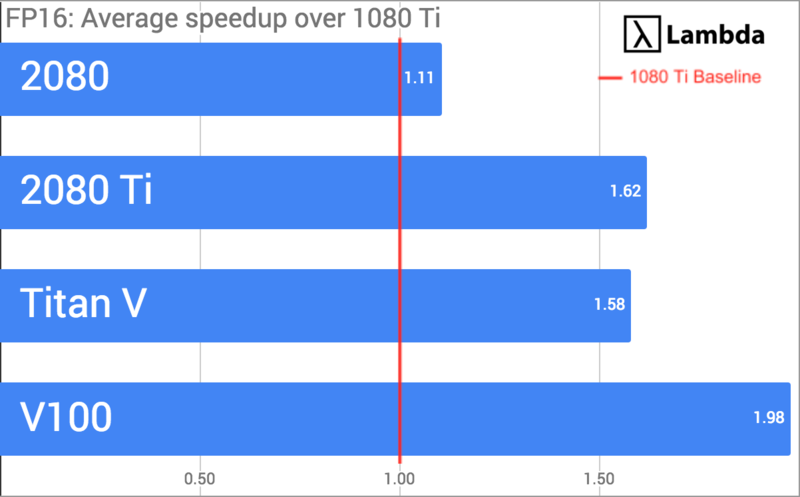
\includegraphics[width=0.65\textwidth]{figures/fp_16_lambda.png}
    \caption{Prestaties van verschillende GPU's, met de NVIDIA GTX 1080 Ti als baseline}
    \label{fig:gpu_performance}
\end{figure}

\subsection{AWS}
De onderstaande prijslijst is afkomstig van Amazon Web Services, dat instanties van cloud computers aanbiedt aan particulieren\footnote{\url{https://aws.amazon.com/ec2/dedicated-hosts/pricing/}}. De P-serie biedt GPU cloud computing instanties aan met NVIDIA Kepler en Volta GPU's.

\begin{table}[H]
    \centering
    \begin{tabular}{c||c|c|c|c|c}
        Model & GPU & vCPU & RAM & GPU RAM & Kosten (per maand) \\
        p2.xlarge & 1 $\times$ NVIDIA Tesla K80 & 4 & 61 & 12 & \$448.22  \\
        p2.8xlarge & 8 $\times$ NVIDIA Tesla V100 & 32 & 488 & 96 & \$3,587.22  \\
        p3.2xlarge & 1 $\times$ NVIDIA Tesla V100 & 8 & 61 & 16 & \$1,524.24 \\
        p3.8xlarge & 4 $\times$ NVIDIA Tesla V100 & 32 & 244 & 64 & \$6,098.42  \\
    \end{tabular}
    \caption{Amazon AWS prijslijst}
    \label{tab:aws_prices}
\end{table}




%%%%%%%%%%%%%%%%%%%%%%%%%%%%%%%%%%%%%%%%%%%%%%%%%%%%%%%%%%%%%%%%%%%%%%%%
\section{Resultaten variant A}
%%%%%%%%%%%%%%%%%%%%%%%%%%%%%%%%%%%%%%%%%%%%%%%%%%%%%%%%%%%%%%%%%%%%%%%%
Variant A heeft de volgende set aan minimale kostenposten voor het ontwikkelen van een prototype:

\begin{table}[H]
    \centering
    \scalebox{0.9}{
        \begin{tabular}{r||c|c|c}
            Onderdeel & Uren & Tarief & Totaal \\
            Standaardnederlandse stem acteur & 24, ca. 7 audioboeken & ca. €2,000 / boek & €14,000 \\
            Speech-to-text herkennings software (IBM) \footnote{\url{https://cloud.ibm.com/docs/services/speech-to-text?topic=speech-to-text-faq-pricing}} & 24 & \$0.48 & \$11.52 \\
            Data preparatie & 40 & €75 & €3,000 \\
            Handmatige orthografische transcriptie & 24 $\times$ 8 (zie: \ref{benodigd_werk}) & €30 & €5,760  \\
            Implementatie Tacotron 2 + WaveGlow & 0 & €0 & €0 \\
            AI engineer (trainen, finetunen netwerk) & 80 (minimaal) & €75 & €3000 \\
            1 $\times$ Getraind netwerk (1k epochs, AWS p3.2xlarge) & 96 & \$3.06 & \$293.76 \\
            \hline
            TOTAAL & 456 & - & €26,065.28 \\
            \hline
            OPTIONEEL & & & \\
            Implementatie SEATS & 80 & €75 & €6,000 \\
            Implementatie Prosody Embedding & 80 & €75 & €6,000 \\
            \hline
            TOTAAL & 160 & - & €12,000 \\
            \hline
            \hline
            TOTAAL & 616 & - & €38,065.28
        \end{tabular}
    }
    \caption{Resultaten variant A}
    \label{tab:resultaat_variant_a}
\end{table}


%%%%%%%%%%%%%%%%%%%%%%%%%%%%%%%%%%%%%%%%%%%%%%%%%%%%%%%%%%%%%%%%%%%%%%%%
\section{Resultaten variant B}
%%%%%%%%%%%%%%%%%%%%%%%%%%%%%%%%%%%%%%%%%%%%%%%%%%%%%%%%%%%%%%%%%%%%%%%%
Variant B heeft de volgende set aan minimale kostenposten voor het ontwikkelen van een prototype:

\begin{table}[H]
    \centering
    \scalebox{0.9}{
        \begin{tabular}{r||c|c|c}
            Onderdeel & Uren & Tarief & Totaal \\
            Standaardnederlandse stem acteur & 24, ca. 7 audioboeken & ca. €2,000 / boek & €14,000 \\
            Speech-to-text herkennings software (IBM) & 24 & \$0.48 & \$11.52 \\
            Data preparatie & 40 & €75 & €3,000 \\
            Handmatige orthografische transcriptie & 24 $\times$ 8 $\times$ 2 (zie: \ref{benodigd_werk}) & €30 & €11,520 \\
            Implementatie Tacotron 2 + WaveGlow & 0 & €0 & €0 \\
            AI engineer (trainen, finetunen netwerk) & 80 (minimaal) & €75 & €3000 \\
            1 $\times$ Getraind netwerk (1k epochs, AWS p3.2xlarge) & 96 & \$3.06 & \$293.76 \\
            \hline
            \hline
            TOTAAL & 648 & - & €31,825.28
        \end{tabular}
    }
    \caption{Resultaten variant B}
    \label{tab:resultaat_variant_b}
\end{table}

%%%%%%%%%%%%%%%%%%%%%%%%%%%%%%%%%%%%%%%%%%%%%%%%%%%%%%%%%%%%%%%%%%%%%%%%
\section{Resultaten variant C}
%%%%%%%%%%%%%%%%%%%%%%%%%%%%%%%%%%%%%%%%%%%%%%%%%%%%%%%%%%%%%%%%%%%%%%%%
Variant C heeft de volgende set aan minimale kostenposten voor het ontwikkelen van een prototype:

\begin{table}[H]
    \centering
    \scalebox{0.9}{
        \begin{tabular}{r||c|c|c}
            Onderdeel & Uren & Tarief & Totaal \\
            Speech-to-text herkennings software (IBM) & 24 & \$0.48 & \$11.52 \\
            Data preparatie & 40 & €75 & €3,000 \\
            Handmatige orthografische transcriptie & 24 $\times$ 8 (zie: \ref{benodigd_werk}) & €30 & €5,760 \\
            Implementatie Tacotron 2 + WaveGlow & 0 & €0 & €0 \\
            AI engineer (trainen, finetunen netwerk) & 80 (minimaal) & €75 & €3000 \\
            1 $\times$ Getraind netwerk (1k epochs, AWS p3.2xlarge) & 96 & \$3.06 & \$293.76 \\
            \hline
            \hline
            TOTAAL & 432 & - & €12,065.28
        \end{tabular}
    }
    \caption{Resultaten variant C}
    \label{tab:resultaat_variant_c}
\end{table}


%%%%%%%%%%%%%%%%%%%%%%%%%%%%%%%%%%%%%%%%%%%%%%%%%%%%%%%%%%%%%%%%%%%%%%%%
\section{Resultaten variant D}
%%%%%%%%%%%%%%%%%%%%%%%%%%%%%%%%%%%%%%%%%%%%%%%%%%%%%%%%%%%%%%%%%%%%%%%%

Variant D heeft de volgende set aan minimale kostenposten voor het ontwikkelen van een prototype:

\begin{table}[H]
    \centering
    \scalebox{0.9}{
        \begin{tabular}{r||c|c|c}
            Onderdeel & Uren & Tarief & Totaal \\
            Implementatie Tacotron 2 + WaveGlow & 0 & €0 & €0 \\
            AI engineer (trainen, finetunen netwerk) & 80 (minimaal) & €75 & €3000 \\
            1 $\times$ Getraind netwerk (1k epochs, AWS p3.2xlarge) & 96 & \$3.06 & \$293.76 \\
            \hline
            TOTAAL & 176 & - & €3,293.76 \\
            \hline
            OPTIONEEL & & & \\
            Implementatie SEATS & 80 & €75 & €6,000 \\
            Implementatie Prosody Embedding & 80 & €75 & €6,000 \\
            \hline
            TOTAAL & 160 & - & €12,000 \\
            \hline
            \hline
            TOTAAL & 336 & - & €15,293.76
        \end{tabular}
    }
    \caption{Resultaten variant D}
    \label{tab:resultaat_variant_d}
\end{table}


%%%%%%%%%%%%%%%%%%%%%%%%%%%%%%%%%%%%%%%%%%%%%%%%%%%%%%%%%%%%%%%%%%%%%%%%
\section{Conclusie}
%%%%%%%%%%%%%%%%%%%%%%%%%%%%%%%%%%%%%%%%%%%%%%%%%%%%%%%%%%%%%%%%%%%%%%%%
Het aanschaffen van een GPU wordt aangeraden wanneer er genoeg ontwikkel- en financiële potentie is om een product te ontwikkelen en die in productie te nemen. Voor het ontwikkelen van een of meerdere prototypes volstaat het huren van een AWS cloud computer.

Alle ontwikkelvarianten, behalve Variant D zonder de optionele implementaties, bedragen meer dan €10,000. Variant A heeft het voordeel dat het ontwikkelen van een Standaardnederlandse stem van hoge kwaliteit, naast dat het gebruikt kan worden als \textit{baseline} om andere stemvarianten te ontwikkelen, an sich een product is dat een potentieel marktaandeel kan bieden voor Prolody B.V. door de huidige schaarste aan volledig bestuurbare, gesynthetiseerde, Nederlandse stemmen van adequate kwaliteit.